\documentclass[article,brazil,english]{techreport}

% ---
% Informações de dados para CAPA e FOLHA DE ROSTO
% ---
\titulo{Applyting the principle of superposition to the design of the magnetic circuit}
\autor{Fábio Pinto Fortkamp}
\local{Florianópolis}
\data{}
\orientador{Prof. Jader Riso Barbosa, Jr.}


% this configures PDF metadata with the above information
\configurepdf

% ---
% compila o indice
% ---
\makeindex
% ---

\usepackage{engsymbols}
\usepackage{magref}


\newcommand{\teslamax}{TeslaMax{ }}
\newcommand{\murm}{\mu_{\mathrm{r},m}}
\newcommand{\indexremmk}{\mathrm{rem},m,k}
\newcommand{\nvbremmk}{\nvb_{\indexremmk}}
\newcommand{\bremmk}{B_{\indexremmk}}
\newcommand{\alpharemmk}{\alpha_{\indexremmk}}


% ----
% Início do documento
% ----

\graphicspath{{../figures/}}
\begin{document}

% Retira espaço extra obsoleto entre as frases.
\frenchspacing 

% ----------------------------------------------------------
% ELEMENTOS PRÉ-TEXTUAIS
% ----------------------------------------------------------
\pretextual

\maketitle

% ----------------------------------------------------------
% ELEMENTOS TEXTUAIS
% ----------------------------------------------------------
\textual

\section{Description of the \teslamax model}
\label{sec:descr-tesl-model}

The \teslamax model is the model for a novel magnetic circuit under development. Its name derive from the goal of maximizing the magnetic flux delivered to the air gap. The first quadrant of the  design can be described by \autoref{fig:teslamax}. 

\begin{figure}[!ht]
  \centering
  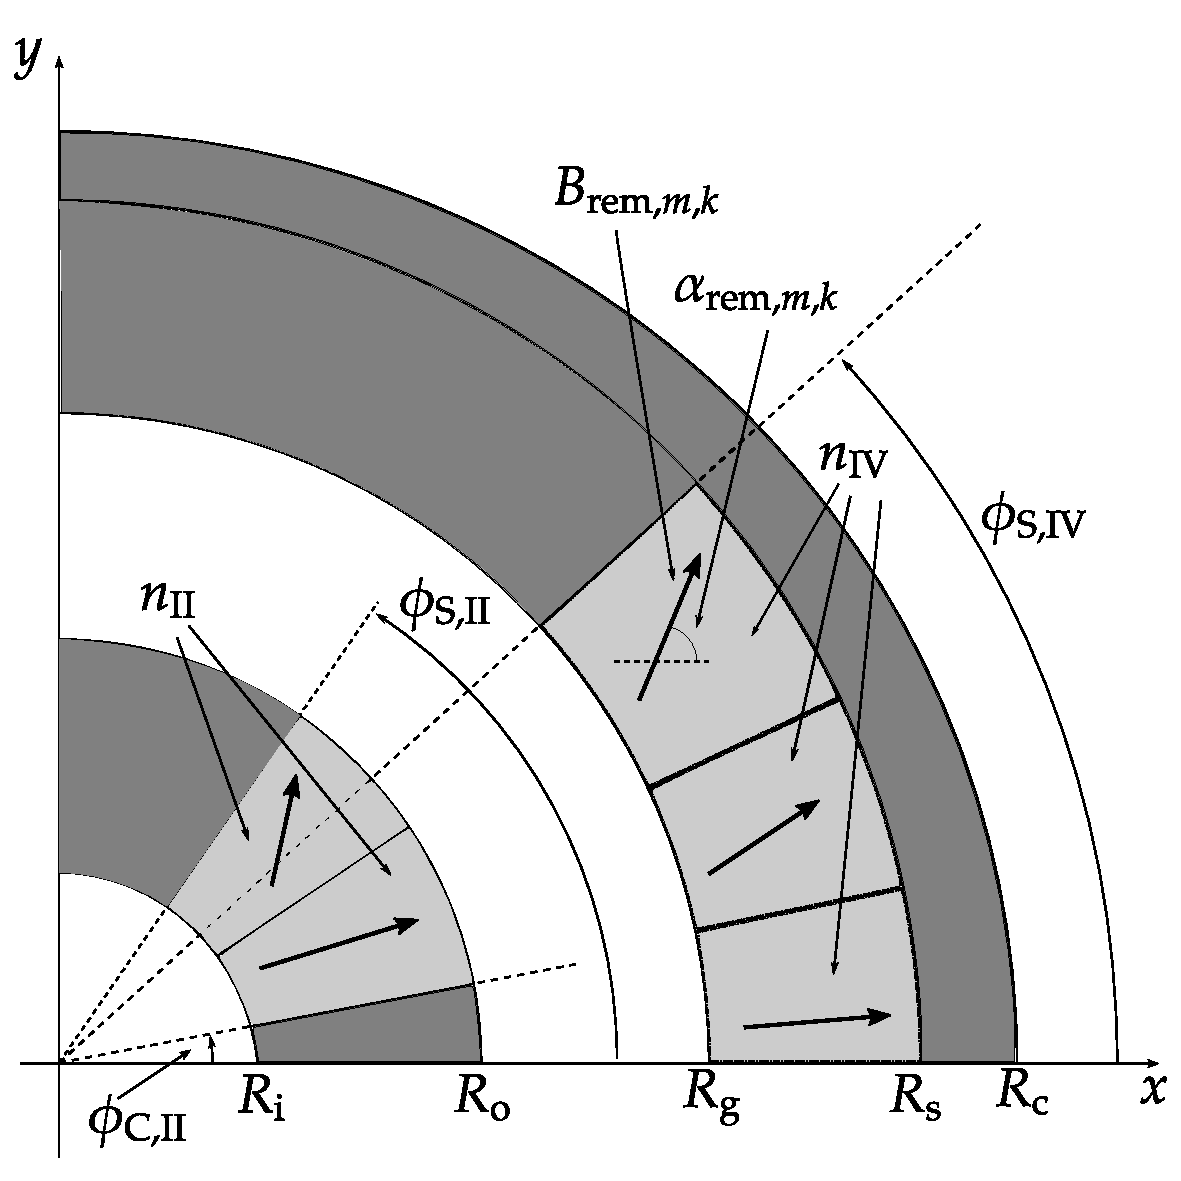
\includegraphics[width=10cm]{teslamax.pdf}
  \caption{Geometry for the \teslamax model. Dark gray areas represent iron, light gray represent permanent magnet, white represent air.}
  \label{fig:teslamax}
\end{figure}

A fundamental feature of \teslamax is that it is composed of an inner and an outer cylinder, denoted by II and IV, respectively. Each cylinder has magnet blocks of equal size (but they may be different across cylinders); there are $n\ped{II}$ blocks in the inner cylinder and $n\ped{IV}$ in the outer one. The segment numbering starts at 1 at the bottom-most unit (lowest value of the $y$-coordinate of the block's center).

All magnet segments are characterized by a relative permeability $\murm$, uniform for magnet $m$; for instance, all blocks in magnet II have permeability $\mu\ped{r,II}$. Each block is uniformily magnetized in a direction:
\begin{equation}
  \label{eq:1}
\nvbremmk = \bremmk \left( \cos\left( \alpharemmk \right) \unitvector{x} + \sin\left( \alpharemmk \right) \unitvector{y} \right)
\end{equation}

\noindent where $m$ represents the magnet and $k$ the segment in that magnet.


Iron blocks fill the remainder of the cylinders, and there is an iron ring outside the outer cylinder. The iron regions are characterized by a relative permeability $\mu\ped{r,iron}$ and have the purpose of guiding the flux lines.

The whole \teslamax system is linear, as will be discussed later.

Only the first quadrant is represented for simplicity; it can be shown that, to maintain a two-pole symmetry, the following conditions must be applied:

\begin{enumerate}
\item The orientation of the remanence vectors in the second quadrant is opposed to the first quadrant:

  \begin{equation}
    \label{eq:2}
    \left( \alpharemmk \right)\ped{1Q} = -\left( \alpharemmk \right)\ped{2Q}
  \end{equation}
\item The top half-circle (first and second quadrant) has mirror symmetry with the bottom one; this \emph{magnetic insulation} condition is equivalent to specifying:

  \begin{equation}
    \label{eq:3}
    \nvb \cdot \normalvector = 0 \quad (y = 0)
  \end{equation}
\end{enumerate}

% ----------------------------------------------------------
% ELEMENTOS PÓS-TEXTUAIS
% ----------------------------------------------------------
\postextual

% ----------------------------------------------------------
% Referências bibliográficas
% ----------------------------------------------------------
\bibliography{refs/Thermo-Foam-Ref}



\end{document}

%%% Local Variables:
%%% mode: latex
%%% TeX-master: t
%%% End:
